%% Run LaTeX on this file several times to get Table of Contents,
%% cross-references, and citations.

\documentclass[11pt]{book}
\usepackage{gvv}
\usepackage{gvv-book-bkup}
%\usepackage{Wiley-AuthoringTemplate}
\usepackage[sectionbib,authoryear]{natbib}% for name-date citation comment the below line
%\usepackage[sectionbib,numbers]{natbib}% for numbered citation comment the above line

%%********************************************************************%%
%%       How many levels of section head would you like numbered?     %%
%% 0= no section numbers, 1= section, 2= subsection, 3= subsubsection %%
\setcounter{secnumdepth}{3}
%%********************************************************************%%
%%**********************************************************************%%
%%     How many levels of section head would you like to appear in the  %%
%%				Table of Contents?			%%
%% 0= chapter, 1= section, 2= subsection, 3= subsubsection titles.	%%
\setcounter{tocdepth}{2}
%%**********************************************************************%%
\setcounter{tocdepth}{3}
%\includeonly{ch01}
\makeindex

\begin{document}

\frontmatter
%%%%%%%%%%%%%%%%%%%%%%%%%%%%%%%%%%%%%%%%%%%%%%%%%%%%%%%%%%%%%%%%
%% Title Pages
%% Wiley will provide title and copyright page, but you can make
%% your own titlepages if you'd like anyway
%% Setting up title pages, type in the appropriate names here:

\booktitle{CBSE Math}

\subtitle{Made Simple}

\AuAff{G. V. V. Sharma}

%% \\ will start a new line.
%% You may add \affil{} for affiliation, ie,
%\authors{Robert M. Groves\\
%\affil{Universitat de les Illes Balears}
%Floyd J. Fowler, Jr.\\
%\affil{University of New Mexico}
%}

%% Print Half Title and Title Page:
%\halftitlepage
\titlepage

%%%%%%%%%%%%%%%%%%%%%%%%%%%%%%%%%%%%%%%%%%%%%%%%%%%%%%%%%%%%%%%%
%%Copyright Page

\begin{copyrightpage}{2023}
%Title, etc
\end{copyrightpage}

% Note, you must use \ to start indented lines, ie,
% 
% \begin{copyrightpage}{2004}
% Survey Methodology / Robert M. Groves . . . [et al.].
% \       p. cm.---(Wiley series in survey methodology)
% \    ``Wiley-Interscience."
% \    Includes bibliographical references and index.
% \    ISBN 0-471-48348-6 (pbk.)
% \    1. Surveys---Methodology.  2. Social 
% \  sciences---Research---Statistical methods.  I. Groves, Robert M.  II. %
% Series.\\

% HA31.2.S873 2004
% 001.4'33---dc22                                             2004044064
% \end{copyrightpage}

%%%%%%%%%%%%%%%%%%%%%%%%%%%%%%%%%%%%%%%%%%%%%%%%%%%%%%%%%%%%%%%%
%% Only Dedication (optional) 

%\dedication{To my parents}

\tableofcontents

%\listoffigures %optional
%\listoftables  %optional

%% or Contributor Page for edited books
%% before \tableofcontents

%%%%%%%%%%%%%%%%%%%%%%%%%%%%%%%%%%%%%%%%%%%%%%%%%%%%%%%%%%%%%%%%
%  Contributors Page for Edited Book
%%%%%%%%%%%%%%%%%%%%%%%%%%%%%%%%%%%%%%%%%%%%%%%%%%%%%%%%%%%%%%%%

% If your book has chapters written by different authors,
% you'll need a Contributors page.

% Use \begin{contributors}...\end{contributors} and
% then enter each author with the \name{} command, followed
% by the affiliation information.

% \begin{contributors}
% \name{Masayki Abe,} Fujitsu Laboratories Ltd., Fujitsu Limited, Atsugi, Japan
%
% \name{L. A. Akers,} Center for Solid State Electronics Research, Arizona State University, Tempe, Arizona
%
% \name{G. H. Bernstein,} Department of Electrical and Computer Engineering, University of Notre Dame, Notre Dame, South Bend, Indiana; formerly of
% Center for Solid State Electronics Research, Arizona
% State University, Tempe, Arizona 
% \end{contributors}

%%%%%%%%%%%%%%%%%%%%%%%%%%%%%%%%%%%%%%%%%%%%%%%%%%%%%%%%%%%%%%%%
% Optional Foreword:

%\begin{foreword}
%\lipsum[1-2]
%\end{foreword}

%%%%%%%%%%%%%%%%%%%%%%%%%%%%%%%%%%%%%%%%%%%%%%%%%%%%%%%%%%%%%%%%
% Optional Preface:

%\begin{preface}
%\lipsum[1-1]
%\prefaceauthor{}
%\where{place\\
% date}
%\end{preface}

% ie,
% \begin{preface}
% This is an example preface.
% \prefaceauthor{R. K. Watts}
% \where{Durham, North Carolina\\
% September, 2004}

%%%%%%%%%%%%%%%%%%%%%%%%%%%%%%%%%%%%%%%%%%%%%%%%%%%%%%%%%%%%%%%%
% Optional Acknowledgments:

%\acknowledgments
%\lipsum[1-2]
%\authorinitials{I. R. S.}  

%%%%%%%%%%%%%%%%%%%%%%%%%%%%%%%%
%% Glossary Type of Environment:

% \begin{glossary}
% \term{<term>}{<description>}
% \end{glossary}

%%%%%%%%%%%%%%%%%%%%%%%%%%%%%%%%
%\begin{acronyms}
%\acro{ASTA}{Arrivals See Time Averages}
%\acro{BHCA}{Busy Hour Call Attempts}
%\acro{BR}{Bandwidth Reservation}
%\acro{b.u.}{bandwidth unit(s)}
%\acro{CAC}{Call / Connection Admission Control}
%\acro{CBP}{Call Blocking Probability(-ies)}
%\acro{CCS}{Centum Call Seconds}
%\acro{CDTM}{Connection Dependent Threshold Model}
%\acro{CS}{Complete Sharing}
%\acro{DiffServ}{Differentiated Services}
%\acro{EMLM}{Erlang Multirate Loss Model}
%\acro{erl}{The Erlang unit of traffic-load}
%\acro{FIFO}{First in - First out}
%\acro{GB}{Global balance}
%\acro{GoS}{Grade of Service}
%\acro{ICT}{Information and Communication Technology}
%\acro{IntServ}{Integrated Services}
%\acro{IP}{Internet Protocol}
%\acro{ITU-T}{International Telecommunication Unit -- Standardization sector}
%\acro{LB}{Local balance}
%\acro{LHS}{Left hand side}
%\acro{LIFO}{Last in - First out}
%\acro{MMPP}{Markov Modulated Poisson Process}
%\acro{MPLS}{Multiple Protocol Labeling Switching}
%\acro{MRM}{Multi-Retry Model}
%\acro{MTM}{Multi-Threshold Model}
%\acro{PASTA}{Poisson Arrivals See Time Averages}
%\acro{PDF}{Probability Distribution Function}
%\acro{pdf}{probability density function}
%\acro{PFS}{Product Form Solution}
%\acro{QoS}{Quality of Service}
%\acro{r.v.}{random variable(s)}
%\acro{RED}{random early detection}
%\acro{RHS}{Right hand side}
%\acro{RLA}{Reduced Load Approximation}
%\acro{SIRO}{service in random order}
%\acro{SRM}{Single-Retry Model}
%\acro{STM}{Single-Threshold Model}
%\acro{TCP}{Transport Control Protocol}
%\acro{TH}{Threshold(s)}
%\acro{UDP}{User Datagram Protocol}
%\end{acronyms}

\setcounter{page}{1}

\begin{introduction}
This book links high school coordinate geometry to linear algebra and matrix analysis through solved problems.

\end{introduction}

\mainmatter

\chapter{Vectors}
\section{2024}
\subsection{12}
\begin{enumerate}
	\item For any two vectors $\overrightarrow{a}$ and $\overrightarrow{b}$, which of the following statements is always true?
		\begin{enumerate}
			\item $\overrightarrow{a} \cdot \overrightarrow{b} \geq |\overrightarrow{a}||\overrightarrow{b}|$
			\item $\overrightarrow{a} \cdot \overrightarrow{b} = |\overrightarrow{a}||\overrightarrow{b}|$
			\item $\overrightarrow{a} \cdot \overrightarrow{b} \leq |\overrightarrow{a}||\overrightarrow{b}|$
			\item $\overrightarrow{a} \cdot \overrightarrow{b} < |\overrightarrow{a}||\overrightarrow{b}|$
		\end{enumerate}
	\item The unit vector perpendicular to both vectors $\hat{i} + \hat{k}$ and $\hat{i} - \hat{k}$ is:
		\begin{enumerate}
			\item $2\hat{j}$
			\item $\hat{j}$
			\item $\frac{\hat{i} - \hat{k}}{\sqrt{2}}$
			\item $\frac{\hat{i} + \hat{k}}{\sqrt{2}}$
		\end{enumerate}
	\item Direction ratios of a vector parallel to line $\frac{x - 1}{2}= -y = \frac{2z + 1}{6}$ are :
		\begin{enumerate}
			\item $2, -1, 6$
			\item $2, 1, 6$
			\item $2, 1, 3$
			\item $2, -1, 3$
		\end{enumerate}
	\item Assertion (A): For two non-zero vectors $\overrightarrow{a}$ and $\overrightarrow{b}$, $\overrightarrow{a} \cdot \overrightarrow{b} = \overrightarrow{b} \cdot \overrightarrow{a}$\\
		Reason (R): For two non-zero vectors $\overrightarrow{a}$ and $\overrightarrow{b}$, $\overrightarrow{a} \times \overrightarrow{b} = \overrightarrow{b} \times \overrightarrow{a}$
		\begin{enumerate}
			\item Both Assertion $(A)$ and Reason $(R)$ are true, and Reason $(R)$ is the correct explaination of Assertion $(A)$.
			\item Both Assertion $(A)$ and Reason $(R)$ are true, but Reason $(R)$ is not the correct explaination of Assertion $(A)$
			\item Assertion $(A)$ is true, but Reason $(R)$ is false
			\item Assertion $(A)$ is false, but Reason $(R)$ is true
		\end{enumerate}
	\item The position vectors of vertices of $\bigtriangleup$ $ABC$ are $A(2\hat{i} - \hat{j} + \hat{k})$, $B(\hat{i} - 3\hat{j} - 5\hat{k})$ and  $C(3\hat{i} - 4\hat{j} - 4\hat{k})$. Find all the angles of $\bigtriangleup$ $ABC$.
\end{enumerate}

\section{2009}
\subsection{12}                              
\begin{enumerate}
\item 
Find the value of $\vec{p}$ if 
$$(2\hat{i} + 6\hat{j} + 27\hat{k}) \times (\hat{i} + 3\hat{j} + p\hat{k}) = \vec{0}.$$

\item 
If $\mathbf{\vec{p}}$ is a unit vector and $(\mathbf{\vec{x}} - \mathbf{\vec{p}}) \cdot (\mathbf{\vec{x}} + \mathbf{\vec{p}}) = 80$, then find $|\mathbf{\vec{x}}|$.
\item 

Find the shortest distance between the following two lines:
$$\vec{r} = (1 + \lambda)\hat{i} + (2 - \lambda)\hat{j} + (\lambda + 1)\hat{k};$$
$$\vec{r} = (2\hat{i} - \hat{j} - \hat{k}) + \mu(2\hat{i} + \hat{j} + 2\hat{k}).$$

\item 
The scalar product of the vector $\hat{i} + \hat{j} + \hat{k}$ with the unit vector along the sum of vectors $2\hat{i} + 4\hat{j} - 5\hat{k}$ and $\lambda \hat{i} + 2\hat{j} + 3\hat{k}$ is equal to one. Find the value of $\lambda$.
\end{enumerate}

%\section{2020}
%\subsection{10}
%\input{2020/vetors1.0.tex}
%\subsection{12}
%\input{2020/vetors2.0.tex}
 
\chapter{linear regression}
\section{2009}
\subsection{12}                                  
\begin{enumerate}
\item A dealer wishes to purchase a number of fans and sewing machines. He has only $\rupee~5,760$ to invest and has a space for at most 20 items.A fan costs him $\rupee~360$ and a sewing machine $\rupee~240$. His expectation is that he can sell a fan at a profit of $\rupee~22$ and a sewing machine at a profit of $\rupee~18$. Assuming that he can sell all the items that he can buy, how should he invest his money in order to maximise the profit ? Formulate this as a linear programming problem and solve it graphically.
\end{enumerate}



\chapter{Linear Forms}
%\section{2023}
%\subsection{10}
%\input{2023/linear-10th.tex}
%\subsection{12}                                                                                                  
%\input{2023/linear-12th.tex}
%\section{2022}

\chapter{Circles}

%\section{2010}
%\subsection{12}
%\input{2010/circles.tex}


\chapter{Intersection of Conics}

%\section{2010}
%\subsection{12}
%\input{2010/intersec.tex}





\chapter{Probability}
\section{2024}
\subsection{12}
\begin{enumerate}
	\item Let $E$ be an event of a sample space $S$ of an experiment, then $P(S|E)=$
		\begin{enumerate}
			\item $P(S \cap E)$
			\item $P(E)$
			\item $1$
			\item $0$
		\end{enumerate}
	\item A pair of dice is thrown simultaneously. If $X$ denotes the absolute difference of the numbers appearing on top of the dice, then find the probability distribution of $X$.
	\item Airplanes are by far the safest mode of transportation when the number of transported passengers are measured against personal injuries and fatality tools.
		\begin{figure}[h]
			\centering
			     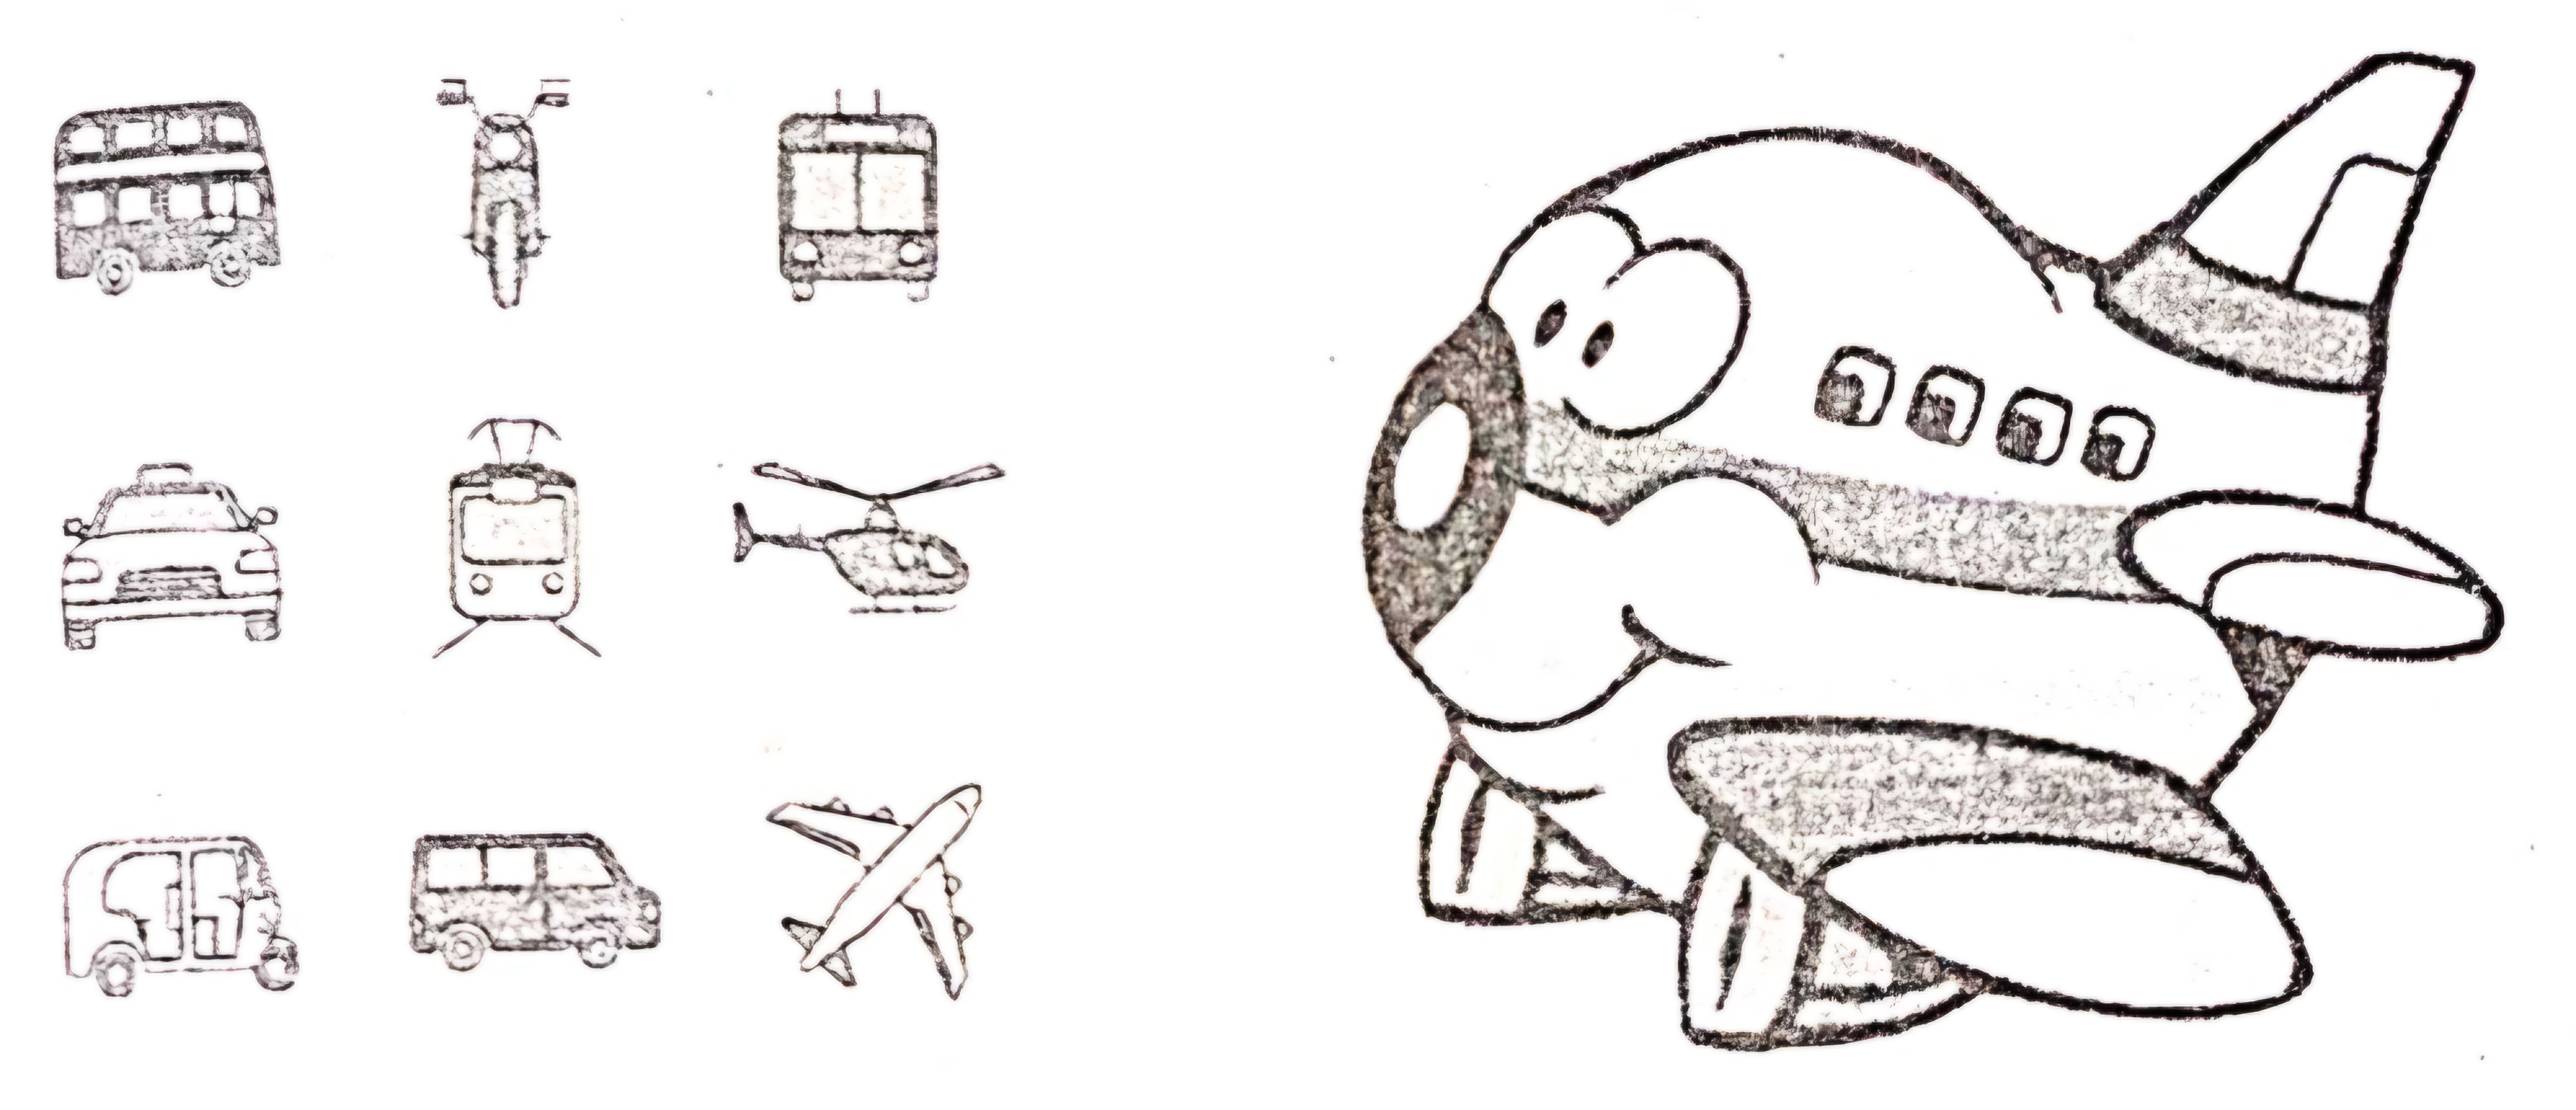
\includegraphics[width=\columnwidth]{figs/Air.jpg}
			     \caption{1}
			\label{Figure}
		\end{figure}
	      Previous records state that the probability of an airplane crash is $0.00001\%$. Further, there are $95\%$ chances that there will be survivors after a plane crash. Assume that in case of no crash, all travellers survive.\\
		Let $E_{1}$ be the event that there is a plane crash and $E_{2}$ be the event that there is no crash. Let $A$ be the event that passengers survive after the journey.\\
	      On the basis of the above information, answer the following questions:
		\begin{enumerate}[label=(\roman*)]
			\item Find the probability that the airplane will not crash.
			\item Find $P(A|E_{1}) + P(A|E_{2})$.
			\item Find $P(A)$
			\item Find $P(E_{2} | A)$.
		\end{enumerate}
\end{enumerate}

\section{2023}
\subsection{10}
\begin{enumerate}
\item A student noted the number of cars passing through a spot on a road for $100$ periods each of $3$ minutes and summarised it in the table given below. Find the mean and median of the following data.\\

	\begin{tabular}{|c|c|c|c|c|c|c|c|c|}
\hline
Number of cars & 0-10 & 10-20 & 20-30 & 30-40 & 40-50 & 50-60 & 60-70 & 70-80\\ 
\hline
Frequency (Periods) & 7 & 14 & 13 & 12 & 20 & 11 & 15 & 8\\ 
\hline

\end{tabular}

\item Computer-based learning $\brak{CBL}$ refers to any teaching methodology that makes use of computers for information transmission. At an elementary school level, computer applications can be used to display multimedia lesson plans. A survey was done on $1000$ elementary and secondary schools of Assam and they were classified by the number of computers they had.

	\begin{figure}[!ht]
		\centering
		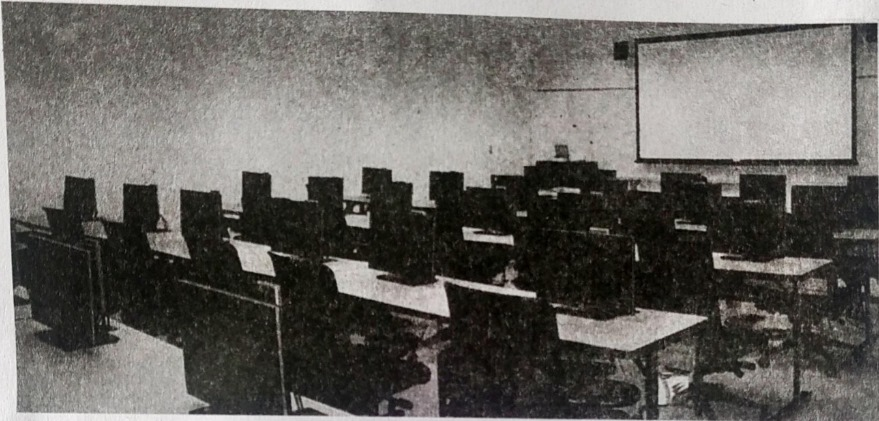
\includegraphics[width=\columnwidth]{figs/last1.jpg}
		\caption{}
		\label{fig:enter-label}
	\end{figure}

	\begin{center}
	\begin{tabular}{|c|c|c|c|c|c|}
	\hline
	\textbf{Number of computers} & 1-10 & 11-20 & 21-50 &  51-100 & 101 and more \\
	\hline
	\textbf{Number of Schools} & 250 & 200 & 290 & 180 & 80 \\
	\hline
	\end{tabular}
	\end{center}

	\text One school is chosen at random.Then:
	\begin{enumerate}
		\item  Find the probability that the school chosen at random has more than $100$ computers.
		\item
		\begin{enumerate}
			\item  Find the probability that the school chosen at random has $50$ or fewer computers.
			\item  Find the probability that the school chosen at random has no more than $20$ computers.
		\end{enumerate}
		\item  Find the probability that the school chosen at random has $10$ or less than $10$ computers.
	\end{enumerate}


\end{enumerate}

\section{2006}
\subsection{10}
\begin{enumerate}

\item A card is drawn at random from a well-shuffled deck of playing cards. Find the probability that the card drawn is

 \begin{enumerate}
        \item a card of spades or an ace
        \item a red king
        \item neither a king nor a queen
        \item either a king or a queen.
 \end{enumerate}

\end{enumerate}


\section{2009}
\subsection{12}                                  
\begin{enumerate}   
\item On a multiple choice examination with three possible answers (out of which only one is correct) for each of the five questions, what is the probability that a candidate would get four or more correct answers just by guessing?  

\item Colored balls are distributed in three bags as shown in the following table:

\begin{table}[h]                                                         
\centering
\scalebox{1.2}{%                                                   
\begin{tabular}{|c|c|c|c|}
\hline                                                              
Bag & \multicolumn{3}{c|}{Colour of the Ball} \\                    
\cline{2-4}                                                         
& Black & White & Red \\                                           
\hline
I & 1 & 2 & 3 \\                                                   
\hline                                                              
II & 2 & 4 & 1 \\                                                  
\hline                                                             
III & 4 & 5 & 3 \\                                                  
\hline
\end{tabular}  
}                                               
\end{table}

A bag is selected at random, and then two balls are randomly drawn from the selected bag. They happen to be black and red. What is the probability that they came from Bag I?

\end{enumerate}

%\section{2010}
%\subsection{12}
%\input{2010/prob.tex}

\chapter{Construction}

%\section{2010}
%\subsection{12}
%\input{2010/construction.tex}


\chapter{Optimization}

%\section{2010}
%\subsection{12}
%\input{2010/opt.tex}


\chapter{Algebra}
\section{2024}
\subsection{12}
\begin{enumerate}
       \item let $f:R_{+} \rightarrow [-5, \infty)$ be defined as $f(x) = 9x^{2} +6x -5$ where $R_{+}$ is the set of all non-negative real numbers, then $f$ is:
	       \begin{enumerate}
		       \item one-one
		       \item onto
		       \item bijective
		       \item neither one-one nor onto
	       \end{enumerate}
       \item The number of points of discontinuity of $f(x) = \begin{dcases}
		       |x|+3, & if x\leq-3  \\
		       -2x, & if -3<x<3 \\
		       6x+2, & if x\geq3 
       \end{dcases}$ is:
		\begin{enumerate}
			\item $0$
			\item $1$
			\item $2$
			\item infinite
		\end{enumerate}
	\item The function $f(x) = x^{3} - 3x^{2} +12x -18$ is:
		\begin{enumerate}
			\item strictly decreasing on $R$
			\item strictly increasing on $R$
			\item neither strictly increasing nor strictly decreasing on $R$
			\item strictly decreasing on $(-\infty, 0)$
		\end{enumerate}
	\item Find the domain of the function $f(x) = \sin^{-1}(x^{2} - 4$. Also, find its range.
	\item If $f(x) = |\tan 2x|$, then find the value of $f'(x)$ at $x=\frac{\pi}{3}$.
	\item If $M$ and $m$ denote the local maximum and local minimum values of the function $f(x) = x + \frac{1}{x} (x\neq0)$ respectively, find the value of $(M-m)$.
	\item Show that $f(x) = e^{x} - e^{-x} + x - \tan^{-1}x$ is strictly increasing in its domain.
	\item Show that a function $f:R \rightarrow R$ defined bt $f(x) = \frac{2x}{1+x ^{2}}$ is neither one-one nor onto. Further, find set $A$ so that the given function $f:R \rightarrow A$ becomes an onto function.
	\item A relation $R$ is defined on $N \times N$ (where $N$ is the set f natural numbers) as:\\
		\centerline{$(a,b)R(c,d) \leftrightarrow a - c = b - d$}\\
	Show that $R$ is an equivalence relation.
        \item The month of September is celebrtaed as the Rashtriya Poshan Maah across the country. Following a healthy and well-balanced diet is crucial in order to supply the body with the proper nutrients it needs. A balanced diet also keeps us mentally fit and promotes improved level of energy.\\
		\begin{figure}[h]
			\centering 
			      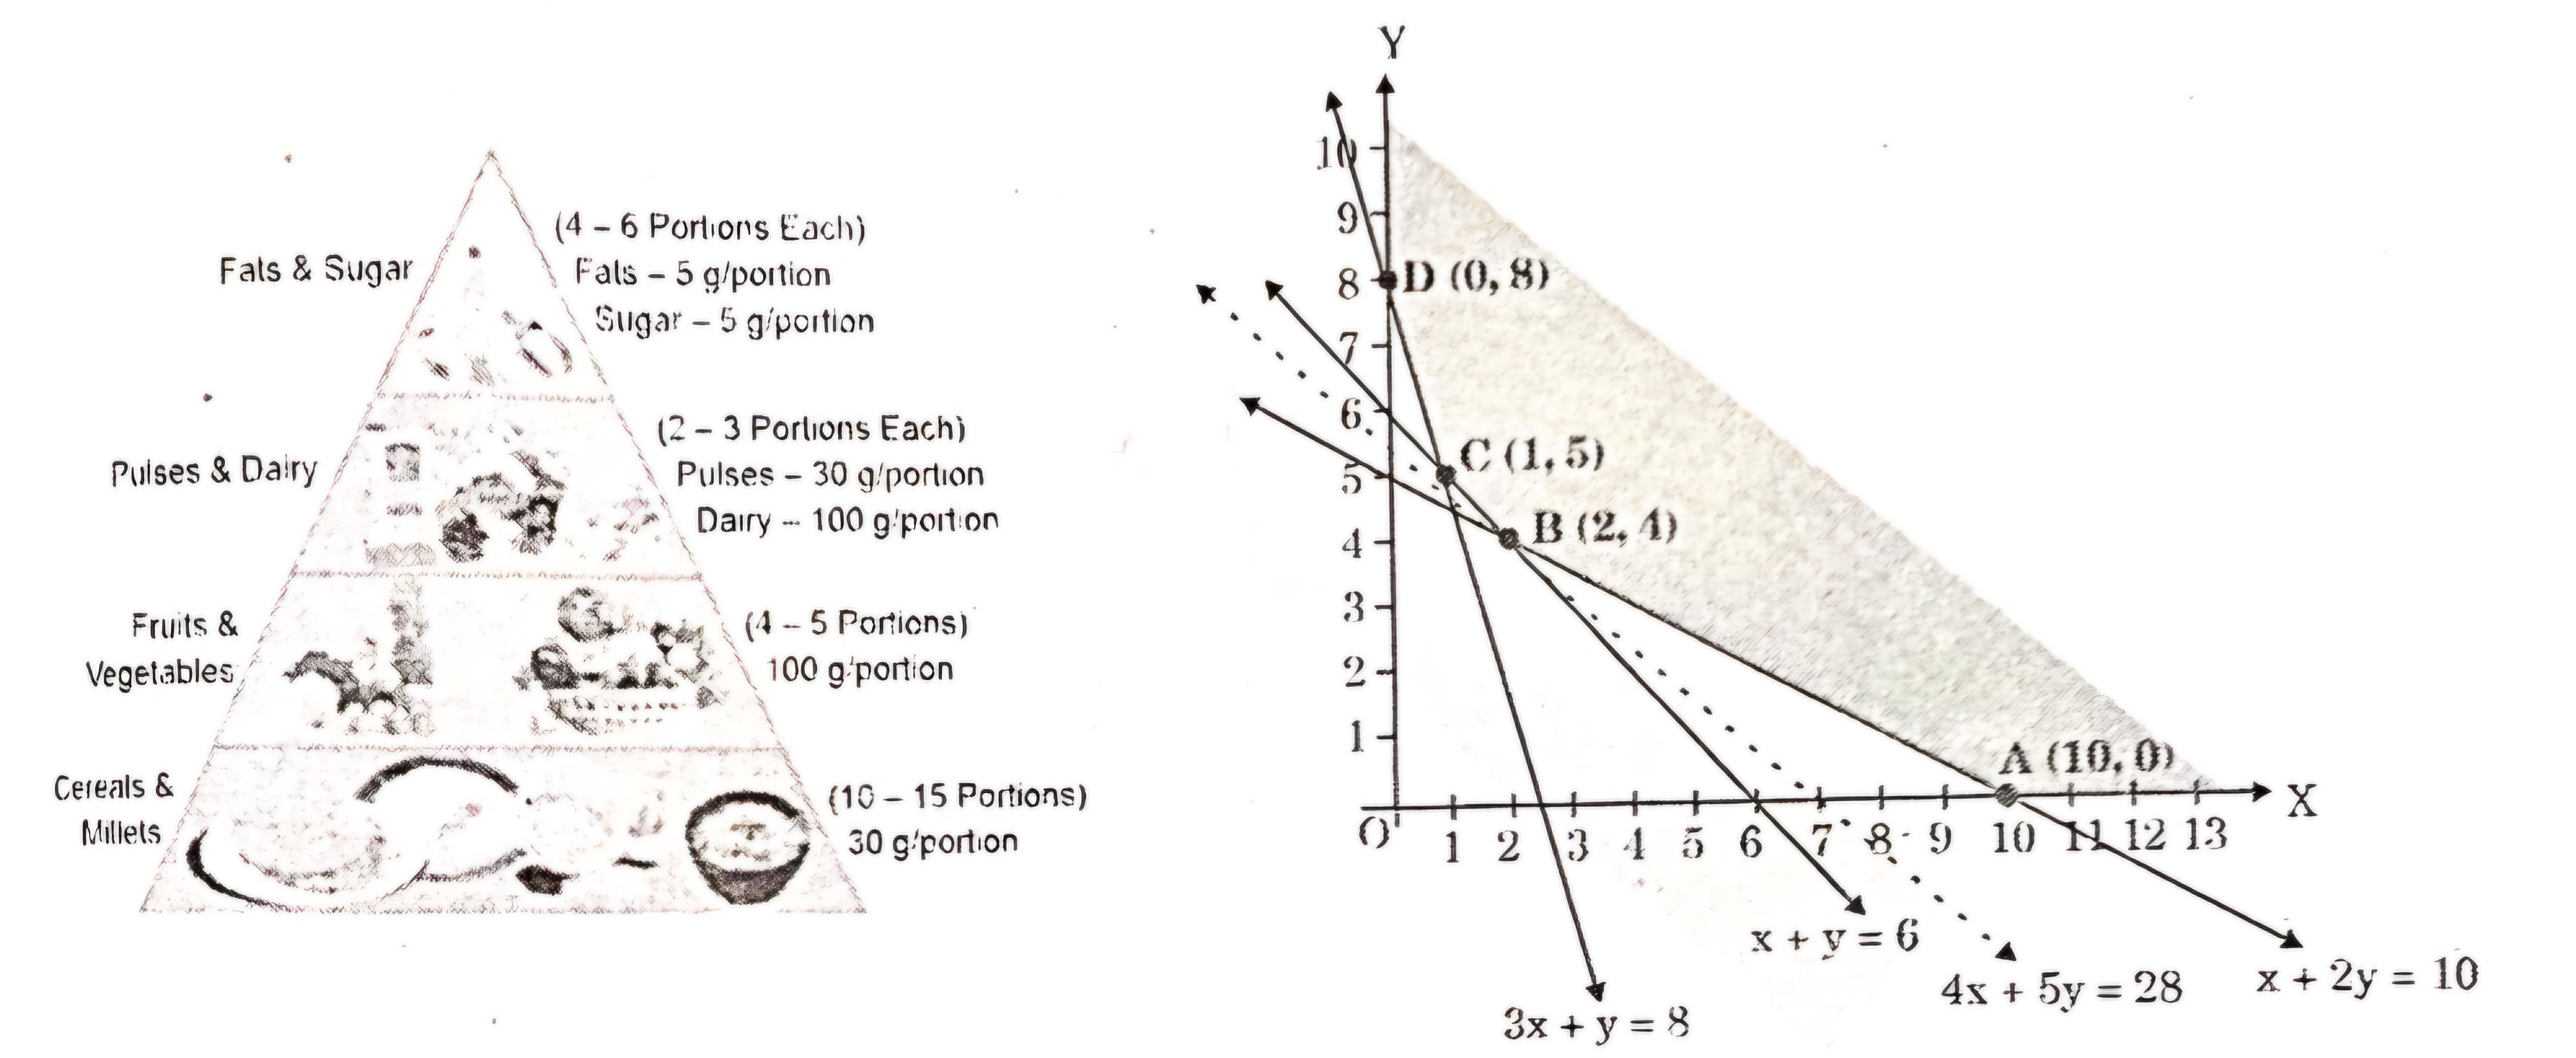
\includegraphics[width=120mm]{figs/Graphs.jpg}
			      \caption{1}
			\label{figure}
		\end{figure}
		A dietician wishes to minimize the cost of a diet involving two types of foods,food $X (x kg)$ and fodd $Y (y kg)$ which are available at the rate of $\rupee 16/kg$ and $\rupee 20/kg$ respectively. The feasible region satisfying the constraints is shown in the graph.\\
		On the basis of the above information, answer the following questions:
		\begin{enumerate}[label=(\roman*)]
			\item Identify and write all the constraints which determine the given feasible region in the above graph.
			\item If the objective is to minimize cost $Z = 16x +20y$, find the values of $x$ and $y$ at which cost is minimum. Also, find minimum cost assuming that minimum cost is possiblr for the given unbounded region.
		\end{enumerate}
\end{enumerate}

\section{2023}
\subsection{10}
\begin{enumerate}
\item \textbf{Assertion (A):}The polynomial p(x)=$x^{2}+3x+3$ has two real zeroes.
	\\\textbf{Reason (R) :} A quadratic polynomial can have at most two zeroes.
\begin{enumerate}
\item Both Assertion (A) and Reason (R) are true and Reason (R) is the correct explanation of Assertion (A). 
\item Both Assertion (A) and Reason (R) are true and Reason (R) is not the correct explanation of Assertion (A).
\item Assertion (A) is true but Reason (R) is false.
\item Assertion (A) is false but Reason (R) is true.
\end{enumerate}

\item Three bells ring at intervals of $ 6, 12 and 18 minutes$. If all the three bells rang at $ 6 a.m.,$ when will they ring together again ?

\item If the system of linear equations  \\ 		
\begin{align}
		2x + 3y = 7 and \\ 
		2ax + \brak{a+b}y = 28
\end{align}
\text have infinite number of solutions, then find the values of $' a '$and$' b '$.

\item If
\begin{align}
	 217x + 131y = 913 and \\
         131x + 217y = 827,
\end{align}
 then solve the equations for the values of $x$ and $y$.

\item How many terms of the arithmetic progression $45,39,33,......$ must be taken so that their sum is $180$? Explain the double answer.
\end{enumerate}


\section{2006}                      
\subsection{10}
\begin{enumerate}
\item \textbf{}Solve the system of equations:

$\frac{bx}{a} - \frac{a y}{b} + a + b = 0 \quad \text{and} \quad b x - a y + 2ab = 0.$

\item Given that:\\

$P$ = $\frac{x+2y}{x+y} + \frac{x}{y}, $Q$=\frac{x+y}{x-y}-\frac{x-y}{x+y}$\quad and $R$=$\frac{x+2y}{x+y}$ - $\frac{x}{x+y}$  \\

\item If $(x + 2)(x - 3)$ is the HCF of the polynomials $p(x) = (x^2 + x - 2)(3x^2 - 8x + c)$ and $q(x) = (x^2 + x - 12)(2x^2 + x + b),$ \\
find the values of $c$ and $b$.

\item  Using the quadratic formula, solve the equation: $A^2 b^2 x^2 - (4b^4 - 3a^4) x - 12 a^2 b^2 = 0.$

\item  A household article is available for \rupee970 cash or \rupee 210 cash down payment followed by three equal monthly installments. If the rate of interest charged under the installment plan is 16\% per annum, find the amount of each installment \\

\item A man borrows \rupee 25,200 from a finance company and has to repay it in two equal annual installments. If the interest is charged at the rate of 10\% per annum compounded annually, calculate the amount of each installment.

\item The speed of a boat in still water is 11 km/hr. It can go 12 km upstream and return 
downstream to the original point in 2 hours 45 minutes. Find the speed of the stream.

\item A bucket made up of a metal sheet is in the form of a frustum of a cone. Its depth is $24\text{ cm}$ and the diameters of the top and bottom are $30\text{ cm}$ and $10\text{ cm}$ respectively. Find the cost of milk which can completely fill the bucket at the rate of \rupee 20 per liter and the cost of the metal sheet used, if it costs \rupee10 per $100\text{ cm}^2$. $(Use \pi=3.14)$


\item Mrs. Ruchi's salary is $\text{Rs.} 32,250$ per month exclusive of HRA. She donates \rupee 12,000 to Prime Minister's Relief Fund ($100\%$ exemption). She also donates \rupee 6,000 to a school and gets a relief of $50\%$ on this donation. She contributes \rupee5,000 per month towards her Provident Fund. She pays a quarterly premium of $\text{Rs.} 2,500$ towards her LIC policy and invests \rupee 25,000 in NSCs. If \rupee 2,700 is the tax deducted each month from her salary for $11$ months, find the tax deducted from her salary in the last month of the year.

\textbf{Income Tax Rates:}

\begin{tabular}{|l|l|}
\hline
Slab & Tax Rate \\
\hline
Up to $\text{Rs.} 1,35,000$ & No tax \\
\hline
From $\text{Rs.} 1,35,001$ to $\text{Rs.} 1,50,000$ & $10\%$ of the taxable income above $\text{Rs.} 1,35,000$ \\
\hline
From $\text{Rs.} 1,50,001$ to $\text{Rs.} 2,50,000$ & $\text{Rs.} 1,500 + 20\%$ of the income exceeding $\text{Rs.} 1,50,000$ \\
\hline
$\text{Rs.} 2,50,001$ and above & $\text{Rs.} 21,500 + 30\%$ of the amount exceeding $\text{Rs.} 2,50,000$ \\
\hline
\end{tabular}

\textbf{Education Cess:} $2\%$ of the income tax


\end{enumerate}

\section{2009}
\subsection{12}                                  
\begin{enumerate}
    \item Let $*$ be a binary operation on $N$ given by $a * b = HCF(a, b)$, where $a, b \in N$. Write the value of $22 * 4$.
    
    \item Let $f : N \rightarrow N$ be a function defined by:
    \[
    f(n) = 
    \begin{cases} 
    \frac{n+1}{2}, & if  n  is odd  \\ 
    \frac{n}{2}, & \text{if } n \text{ is even}
    \end{cases}
    \]
    for all $n \in N$. Find whether the function $f$ is bijective.
    \item A manufacturer can sell $x$ items at a price of Rs. $\left(5 - \frac{x}{100}\right)$ each. The cost price of $x$ is Rs. $\left(\frac{x}{5} + 500\right)$. Find the number of items he should sell to earn maximum profit.
    
    \item Find the intervals in which the function $f$ given by:
\begin{align}
    f(x) = \sin x + \cos x, \quad 0 \leq x \leq 2\pi,
\end{align}
    is strictly increasing or strictly decreasing.
\end{enumerate}





%\section{2010}
%\subsection{12}
%\begin{enumerate}
    \item Let $*$ be a binary operation on $N$ given by $a * b = HCF(a, b)$, where $a, b \in N$. Write the value of $22 * 4$.
    
    \item Let $f : N \rightarrow N$ be a function defined by:
    \[
    f(n) = 
    \begin{cases} 
    \frac{n+1}{2}, & if  n  is odd  \\ 
    \frac{n}{2}, & \text{if } n \text{ is even}
    \end{cases}
    \]
    for all $n \in N$. Find whether the function $f$ is bijective.
    \item A manufacturer can sell $x$ items at a price of Rs. $\left(5 - \frac{x}{100}\right)$ each. The cost price of $x$ is Rs. $\left(\frac{x}{5} + 500\right)$. Find the number of items he should sell to earn maximum profit.
    
    \item Find the intervals in which the function $f$ given by:
\begin{align}
    f(x) = \sin x + \cos x, \quad 0 \leq x \leq 2\pi,
\end{align}
    is strictly increasing or strictly decreasing.
\end{enumerate}






\chapter{Geometry}
\section{2024}
\subsection{12}
\begin{enumerate}
	\item The coordinates of the foot of the perpendicular drawn from the point $(0,1,2)$ on th $x$-axis are given by:
		\begin{enumerate}
			\item $(1,0,0)$
			\item $(2,0,0)$
			\item $(\sqrt{5},0,0)$
			\item $(0,0,0)$
		\end{enumerate}
	\item If a line makes an angle of $30^{\circ}$ with the positive direction of $x$-axis, $120^{\circ}$ with the positive direction of $y$-axis, then the angle which it makes with the positive direction of $z$-axis is:
		\begin{enumerate}
			\item $90^{\circ}$
			\item $120^{\circ}$
			\item $60^{\circ}$
			\item $0^{\circ}$
		\end{enumerate}
	\item Find the equation of the line which bisects the line segment joining points $A(2,3,4)$ and $B(4,5,8)$ and is perpendicular to the lines $\frac{x-8}{3} = \frac{y+19}{-16} = \frac{z-10}{7}$ and $\frac{x-15}{3} = \frac{y-29}{8} = \frac{z-5}{-5}$
	\item If $A_{1}$ denotes the area of region bounded by $y^{2} = 4x$ and $x$-axis in the first quadrant and $A_{2}$ denotes the area of region bounded by $y^{2} = 4x$, $x=4$, find $A_{1} : A_{2}$.
\end{enumerate}

\section{2023}
\subsection{10}

\begin{enumerate}

\item A car has two wipers which do not overlap. Each wiper has a blade of length $21 \mathrm{cm}$ sweeping through an angle of $120\degree$. Find the total area cleaned at each sweep of the two blades.

\item Sides $AB$ and $BC$ and median $AD$ of a triangle $ABC$ are respectively proportional to sides $PQ$ and $QR$ and median $PM$ of $\triangle PQR$.Show that $\triangle ABC \sim \triangle PQR$.

\item Through the mid-point $M$ of the side $CD$ of a parallelogram $ABCD$,the line $BM$ is drawn intersecting $AC$ in $L$ and $AD$ (produced) in $E$.Prove that $EL = 2BL$. 

\item In the given figure, $O$ is the center of the circle .$AB$ and $AC$ are tangents drawn to the circle from point $A$. If $\angle BAC = 65\degree $, then find the measure of $\angle BOC $.
	\begin{figure}[!ht]
		\centering
		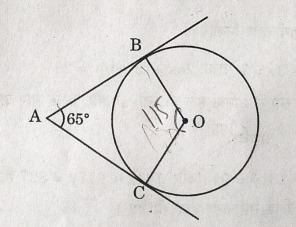
\includegraphics[width=\columnwidth]{figs/last5.jpg}
		\caption{}
		\label{fig:enter-label}
	\end{figure}

\newpage
\item In the given figure, $O$ is the centre of the circle and $QPR$ is a tangent to it at $P$.Prove that $\angle QAP + \angle APR = 90\degree$.

	\begin{figure}[!ht]
		\centering
		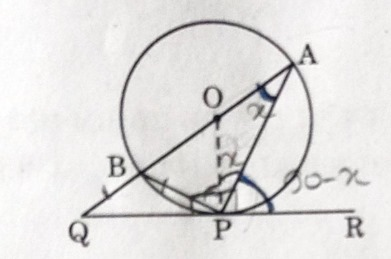
\includegraphics[width=\columnwidth]{figs/last4.jpg}
		\caption{}
		\label{fig:enter-label}
	\end{figure}
\newpage
\item In an annual day function of a school, the organizers wanted to give a cash prize along with a memento to their best students.Each memento is made as shown in the figure and its base $ABCD$ is shown from the front side.The rate of silver plating \rupee~20 $per  \mathrm{cm}^2$.

	\begin{figure}[!ht]
		\centering
		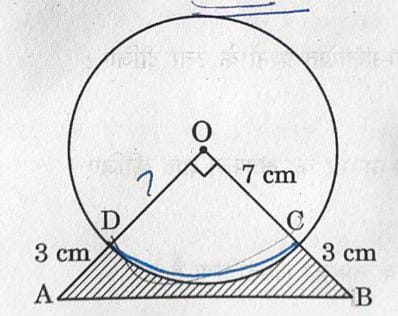
\includegraphics[width=\columnwidth]{figs/last3.jpg}
		\caption{}
		\label{fig:enter-label}
	\end{figure}

	\text Based on the above, answer the following question:
		\begin{enumerate}
			\item What is the area of the quadrant $ODOC$?
			\item Find the area of $\triangle AOB$.
			\item
			\begin{enumerate}
				\item What is the total cost of silver plating the shaded part $ABCD$?
				\item What is the length of arc $CD$ ?
			\end{enumerate}
		\end{enumerate}
\newpage
\item In a coffee shop, coffee is served in two types of cups.One is cylindrical  in shape with diameter $7 \mathrm{cm}$ and height $14 \mathrm{cm} $ and the other is hemispherical with diameter $21 \mathrm{cm}$.

	
	\begin{figure}[!ht]
		\centering
		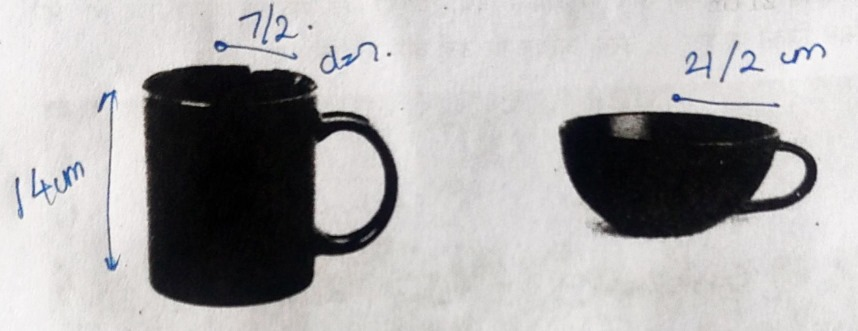
\includegraphics[width=\columnwidth]{figs/last2.jpg}
		\caption{}
		\label{fig:enter-label}
	\end{figure}

	\text Based on the above, answer the following question:
	\begin{enumerate}
		\item  Find the area of the cylindrical cup.
		\item
		\begin{enumerate}
			\item  What is the capacity of the hemispherical cup?
			\item Find the capacity of the cylindrical cup.
		\end{enumerate}
		\item   What is the curved surface area of the cylindrical cup?
         \end{enumerate}

\newpage	
\item Show that the points $\brak{-2,3}, \brak{8,3}$ and $\brak{6,7} $ are the vertices of a right-angled triangle.

\item If $Q\brak{0,1}$ is equidistant from $P\brak{5,-3}$ and $R\brak{x,6}$,find the values of $x$.


\end{enumerate}


\section{2006}
\subsection{10}
\begin{enumerate}
\item In Figure 1, $\angle BAC = 90^\circ$. $AD$ $\parallel$ $BC$. Prove that $AB^2 + CD^2 = BD^2 + AC^2$.
        \begin{figure}[h]
        \centering
                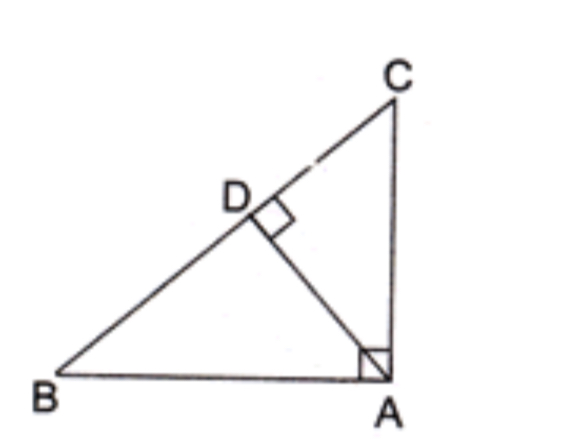
\includegraphics[width=70mm]{figs/IMG01.PNG}
                \caption{1}                                                                                               \label{fig}                   
         \end{figure}
\item  In Figure 2, $PT = 6 \text{ cm}$, $AR = 5 \text{ cm}$. Find the length of $PA$.

\begin{figure}[h]
        \centering
                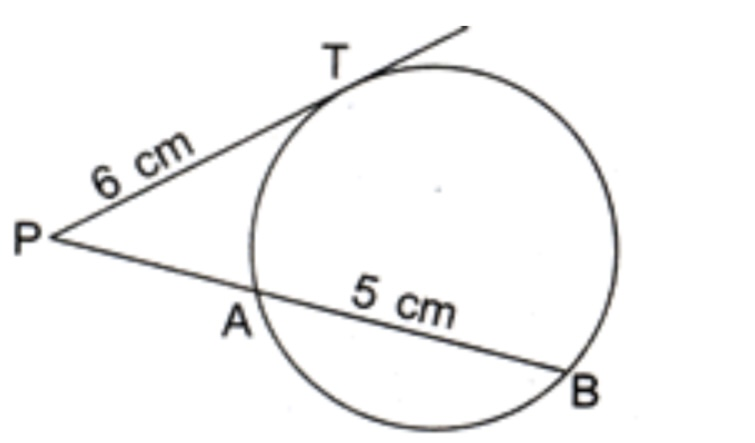
\includegraphics[width=70mm]{figs/IMG02.PNG}
                \caption{2}
                \label{fig:}
\end{figure}

                                                             \item Draw the graphs of the following equations:
$3x - 4y + 6 = 0 ,3x + y - 9 = 0$
Also, determine the co-ordinates of the vertices of the triangle formed by these lines and the x
axis.
\item  A solid is in the form of a right circular cylinder with hemispherical ends. The total height
of the solid is 58 cm and the diameter of the cylinder is 28cm. Find the total surface area of the
   solid  $\pi \approx \frac{22}{7} $

\item . Construct a triangle $ABC$ in which $BC$ = 7 cm, and median $AD$ = 5 cm, $\angle A=60^\circ$ Write      the steps of construction also.

\begin{figure}[h]                                                                                                 \centering
                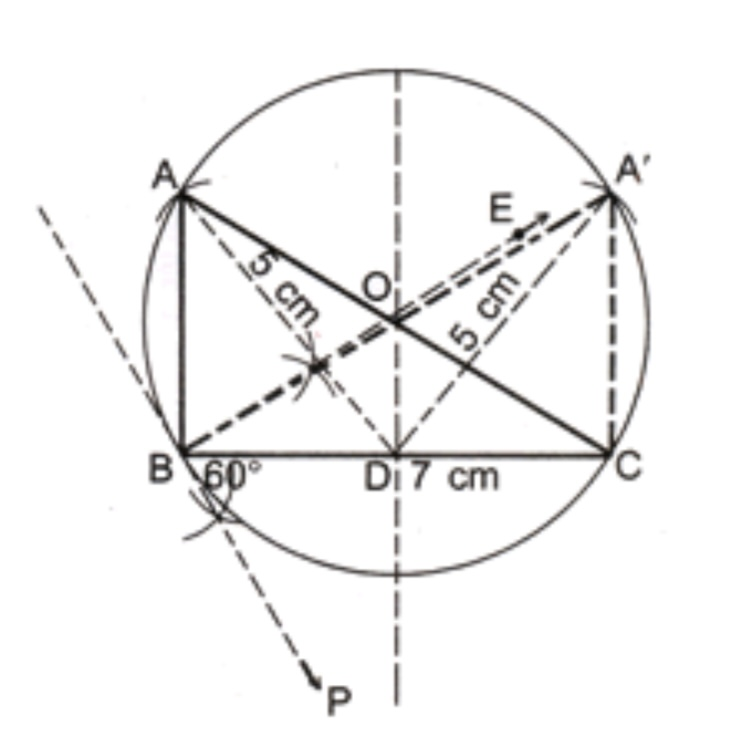
\includegraphics[width=70mm]{figs/IMG04.PNG}                                                     \caption{3}
                 \label{fig:}                                                                       \end{figure}.
\item Show that the points A(6, 2), B(2, 1), C(1, 5) and D(5, 6) are the vertices of a square

\item Find the value of p for which the points (- 5, 1), (1, p) and \(4, - 2\) are collinear.
\item . Prove that in a right triangle, the square of the hypotenuse is equal to the sum of the
squares of the other two sides.
\begin{figure}[h]
        \centering
          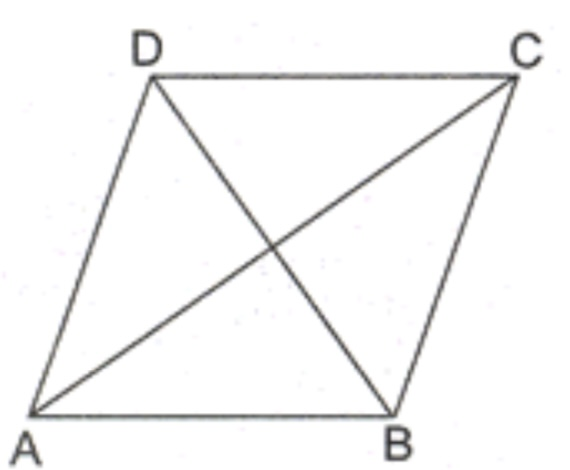
\includegraphics[width=70mm]{figs/IMG03.PNG}
          \caption{4}                                                                                                                                             \label{fig:}

 \end{figure}\\
Makeing  ue  of the above, prove the following:\\
in fig:4, $ABCD$ is a fig:4 rhombus. prove that $4AB^2 =  AC^2 +BD^2$.


\item Prove that I a line touch a circle and from the point of contact a chord is drawn, the angles
which this chord makes with the given line are equal respectively to the angles formed in the
corresponding alternate segments.
Using the above, do the following: \\
$AB$ is a diameter and $AC$ is a chord of a circle such that $\angle BAC=30^\circ$. The tangent at C
intersects $AR$ produced in a point I Prove that $BC = RD.$

\item A man standing on the deck of a ship, which is 10 m above the water level, observes the
angle of elevation of the top of a hill as 60° and the angle of depression of the base of the hill as
300. Calculate the distance of the hill from the ship and the height of the hill.

\item From a window $x$ meters high above the ground in a street, the angles of elevation and depression of the top and foot of the other house on the opposite side of the street are $\alpha$ and $\beta$ respectively. Show that the height of the opposite house is $x(1 + \tan \alpha \cot \beta)$ meters.






\end{enumerate}

\section{2009}
\subsection{12}                                  
\begin{enumerate}
\item 
Write the direction cosines of a line equally inclined to the three coordinates axes. 
\item 
Find the equation of the plane determined by the points $A(3, -1, 2), B(5, 2, 4)$ and $C(-1, -1, 6)$. also find the distance of the point $P(6, 5, 9)$ from the plane.
\item 
Find the area of the region included between the parabola ${y}^ {2} = x$ and the line $x + y = 2$
\item 
The length $x$ of a rectangle is decreasing at the rate of $5 cm$/minute and the width $y$ is increasing at the rate of $4 cm$/minute. When $x = 8 cm $and$ y = 6 cm$, find the rate of change of $(a)$ the perimeter,$ (b)$ the area of the rectangle.
\end{enumerate}



%\section{2023}
%\subsection{10}
%\input{2023/ASSIGNMENT_1.tex}

\chapter{sequences}
\section{2006}                       
\subsection{10}

\begin{enumerate}
    \item The $5^{\text{th}}$ term of an Arithmetic Progression (A.P.) is 26 and the 10th term is 51. Determine the $15^{\text{th}}$ term of the A.P.
    \item Find the sum of all the natural numbers less than 100 which are divisible by 6.
\end{enumerate}




\chapter{Datahandling}
\section{2006}
\subsection{10}
\begin{enumerate}
\item The following table shows the monthly expenditure of company. Draw apie chart for the data.

\begin{tabular}{|l|c|}
\hline
\ & Amount (in Rs.) \\
\hline
Wages & 4800 \\
Materials & 3200 \\
Taxation & 2400 \\
Adm. Expenditure & 3000 \\
Miscellaneous & 1000 \\
\hline
\end{tabular}


\item The Arithmetic Mean of the following frequency distribution is 47. Determine the value of $p$.
\begin{tabular}{|c|c|}
\hline
Classes & Frequency \\
\hline
0 - 20 & 8 \\
20 - 40 & 15 \\
40 - 60 & 20 \\
60 - 80 & $p$ \\
80 - 100 & 5 \\
\hline
\end{tabular}



\end{enumerate}





\chapter{Discrete}
%\section{2010}
%\subsection{12}
%\input{2010/discrete.tex}

\chapter{Number Systems}
\section{2023}
\subsection{10}

\begin{enumerate}

\item Prove that $ 2+\sqrt3 $ is an irrational number,given that $ \sqrt3 $ is an irrational number.

\item Find by prime factorisation the $LCM$ of the number $18180$ and $7575$. Also,find the $HCF$ of the two numbers.


\end{enumerate}


%\section{2010}
%\subsection{12}
%\input{2010/numbersys.tex}


\chapter{Differentiation}
\section{2024}
\subsection{12}
\begin{enumerate}
	\item The derivative of $\tan^{-1}(x^{2})$ w.r.t. $x$ is:
		\begin{enumerate}
			\item $\frac{x}{1 + x^{4}}$
			\item $\frac{2x}{1 +x^{4}}$
			\item $-\frac{2x}{1 + x^{4}}$
			\item $\frac{1}{1+x^{4}}$
		\end{enumerate}
	\item Overspeeding increases fuel consumption and decreases fuel economy as a result of tyre rolling friction and air resistance. While vehicles reach optimal fuel economy at different speeds, fuel mileage usualy decreases rapidly at speeds above 80km/h. \\
		\begin{figure}[h]
			\centering
			      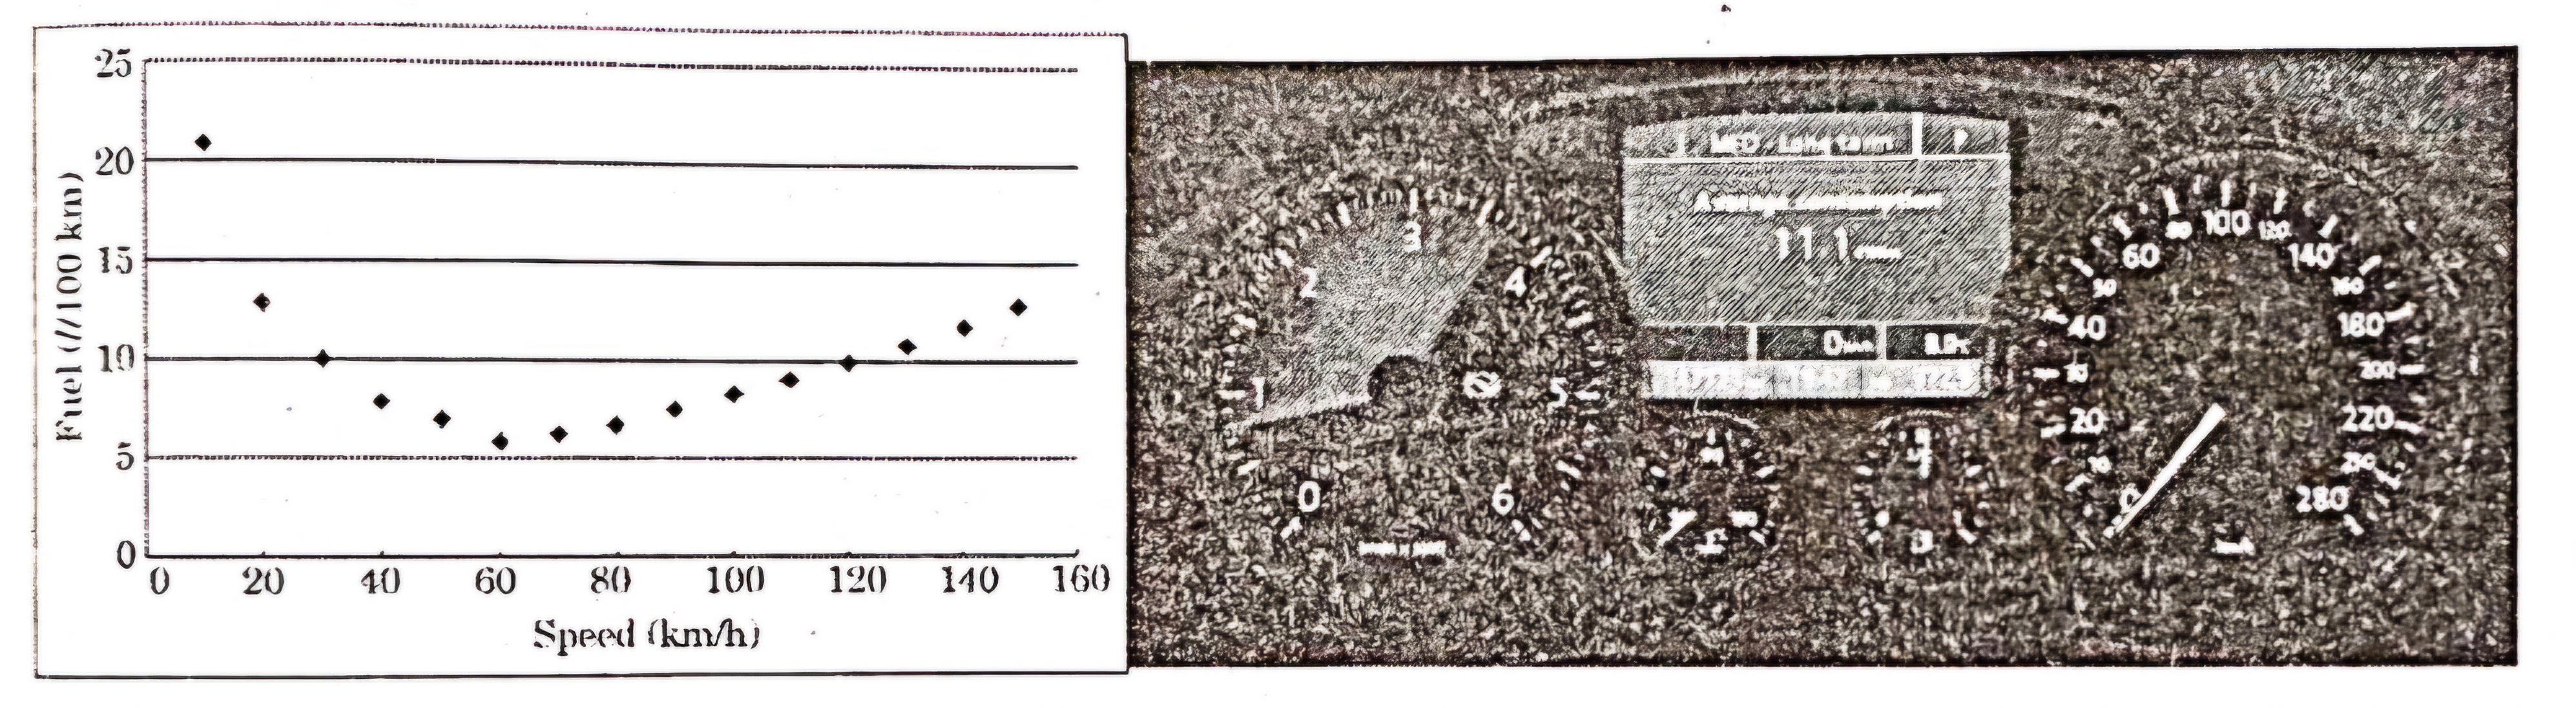
\includegraphics[width=120mm]{figs/Speed.jpg}
			      \caption{1}
			\label{Figure}
		\end{figure}
		The relation btween fuel consumption F(l/100 km) and speed V(km/h) under some constraints is given as $F = \frac{V^{2}}{500} - \frac{V}{4} +14$. \\
		On the basis of the above information, answer the following questions:
		\begin{enumerate}[label=(\roman*)]
			\item  Find F, when $V = 40km/h$.
			\item  Find $\frac{dF}{dV}$.
			\item  Find he speed V for which fuel consumption F is minimum.
			\item  Find the quantity of fuel required to travel 600 km at the speed V at which $\frac{dF}{dV} = -0.01$.
		\end{enumerate}
\end{enumerate}

\begin{enumerate}
	\item The differential equation $\frac{dy}{dx}=F(x,y)$ will not be a homogeneous differential equation, if $F(x,y)$ is:
		\begin{enumerate}
			\item $\cos x - \sin (\frac{y}{x})$
			\item $\frac{y}{x}$
			\item $\frac{x^{2} + y^{2}}{xy}$
			\item $\cos^{2}(\frac{x}{y})$
		\end{enumerate}
	\item The degree of the differential equation $(y'')^{2} + (y')^{3} = x\sin(y')^{3}$ is:
		\begin{enumerate}
			\item $1$
			\item $2$
			\item $3$
			\item not defined
		\end{enumerate}
	\item If $y=\cosec (\cot^{-1} x)$, then prove that $\sqrt{1 + x^{2}} \frac{dy}{dx} -x = 0$.
	\item If $x=e^{\cos 3t}$ and $y=e^{\sin 3t}$, prove that $\frac{dy}{dx} = -\frac{ylogx}{xlogy}$.
	\item Show that: $\frac{d}{dx} (|x|)=\frac{x}{|x|}, x\neq0$.
	\item  Find the particular solution of the differetial equation given by $2xy + y^{2} - 2x^{2} \frac{dy}{dx} = 0; y=2$, when x=1.
	\item Find the general solution of the differential equation:\\
		\centerline {$ydx = (x + 2y^{2})$dy}
\end{enumerate}

\section{2009}
\subsection{12}                                  
\begin{enumerate}
    \item if $\sin y = x \sin(a + y),$ prove that $\frac{dy}{dx} = \frac{sin^2(a+y)}{\sin a}.$
    \item if $(\cos x)^y = (sin y)^x, $ find $\frac{dy}{dx}.$
    \item if $y = \frac{sin^{-1} x}{\sqrt{1-x^2}}$, show that
    \item $(1 - x^2)\frac{d^2{y}}{dx^2}-3x\frac{dy}{dx} - y = 0$
    \item Solve the following differential equation :
    
    \hspace{20pt} $x \frac{dy}{dx} = y - x \tan \frac{y}{x}$

    \item solve the following differential equation :

    \hspace{20pt} ${cos^{2}} {x} \frac{dy}{dx} + y = \tan x$


    
\end{enumerate}



%\section{2023}
%\subsection{12}
%\input{2023/differentiation.tex}






\chapter{Integration}
\section{2024}
\subsection{12}
\begin{enumerate}
	\item $\int\limits_0^{\frac{\pi}{2}} \frac{\sin x - \cos x}{1 + \sin x\cos x}dx$ is equal to:
		 \begin{enumerate}
			 \item $\pi$
			 \item $Zero(0)$
			 \item $\int\limits_0^{\frac{\pi}{2}}$ $\frac{2\sin x}{1+ \sin x\cos x}dx$
			 \item $\frac{\pi^{2}}{4}$
		 \end{enumerate}
	 \item Find : $\int \frac{e^{4x}-1}{e^{4x}+1}dx$
	 \item Evaluate:\\
		 $\int\limits_{2}{-2} \sqrt{\frac{2-x}{z+x}}dx$ 
	 \item Find: \\
		$\int \frac{1}{x[(logx)^{2} - 3logx - 4]}dx$
	\item Find: $\int x^{2} \cdot \sin^{-1} (x^{\frac{3}{2}})dx$ 
\end{enumerate}

\section{2009}
\subsection{12}                              
\begin{enumerate}
\item Evaluate:
    
\hspace{39pt} $\int\limits_{0}^{\frac{1}{\sqrt{2}}} \frac{1}{\sqrt{1 - x^2}}$ \, dx 
   

\item Evaluate:\\
    
\hspace{39pt} $\int\frac{cos\sqrt{x}}{\sqrt{x}}$\, dx\\
    
\item Evaluate:\\
    
\hspace{39pt}$\int \frac{dx}{\sqrt{5-4x-2x^2}}$ \\
\vspace{10pt}
\item Evaluate:\\

\hspace{39pt}$\int x sin^{-1}{x}\,dx$\\
    

\item Evaluate:\\
    
\hspace{39pt} $\int\limits_{0}^{\pi}\frac{x dx}{a^2 \cos^2 x + b^2 \sin^2 x}$ \\
\vspace{10pt}
    
\hspace{39pt} $\int\limits_{0}^{\pi} \frac{x dx}{a^2 \cos^2 x + b^2 \sin^2 x}$ \\

\end{enumerate}




%\section{2010}
%\subsection{12}
%\input{2010/integrate.tex}


\chapter{Functions}
%\section{2023}
%\subsection{12}
%\input{2023/Functions.tex}




\chapter{Matrices}
\section{2024}
\subsection{12}
\begin{enumerate}
    \item If the sum of all the elements of $3 \times 3$ scalar matrix is $9$, then the product of all elements is:
	    \begin{enumerate}
		    \item $0$
		    \item $9$
		    \item $27$
		    \item $729$
	    \end{enumerate}
    \item If $ \mydet{-a & b & c\\a & -b & c\\a & b & -c} = kabc$, then the value of $k$ is:
	    \begin{enumerate}
		    \item $0$
		    \item $1$
		    \item $2$
		    \item $4$
	    \end{enumerate}
    \item If $A=[a_{ij}]$ be a $3 \times 3$ where $a_{ij} = i - 3j$,then which of the following is false?
	    \begin{enumerate}
		    \item $a_{11}<0$
		    \item $a_{12} +a_{21} = -6$
		    \item $a_{13}>a_{31}$
		    \item $a_{31}=0$
	    \end{enumerate}
    \item If $F(x)= \myvec{\cos x & -\sin x & 0\\ \sin x & \cos x & 0\\ 0 & 0 &0}$ and $[F(x)]^2$=$F(kx)$, then the value of $k$ is:
	    \begin{enumerate}
		    \item $1$
		    \item $2$
		    \item $0$
		    \item $-2$
	    \end{enumerate}
    \item Assertion (A): For any symmetric matrix $A$, $B'AB$ is a skew-symmetric matrix.\\
	  Reason (R): A square matrix $P$ is kew-symmetric if $P'=-P$
		\begin{enumerate}
			\item Both Assertion and Reason are true, and Reason is the correct explaination of Assertion.
			\item Both Assertion and Reason are true, but Reason is not the correct explaination of Assertion.
			\item Assertion is true, but Reason is false.
			\item Assertion is false, but Reason is true.
		\end{enumerate}
	\item Solve the following system of equations,using matrices:\\
		$\frac{2}{x} + \frac{3}{y} + \frac{10}{z}  = 4$, $\frac{4}{x} - \frac{6}{y}  + \frac{5}{z} =1$, $\frac{6}{x} + \frac{9}{y} - \frac{20}{z} = 2$ where $x,y,z \neq 0$\\
	\item If $A= \myvec{1 & \cot x\\ -\cot x & 1}$,then show that $A'A^-1= \myvec{-\cos 2x & -\sin 2x \\ \sin 2x & -\cos 2x}$
\end{enumerate}

\section{2009}
\subsection{12}
\begin{enumerate}
	\item Find the value of $x$, if \\
		$\myvec{3x+y & -y\\ 2y-x &3} = \myvec{1 & 2\\ -5 & 3}$.
	\item Write the value of the following determinant:\\
		\centerline{$\mydet{a-b & b-c & c-a\\ b-c & c-a & a-b\\ c-a & a-b & b-c}$}
	\item Find the value of $x$ from the following:\\
		\centerline{$\mydet{x & 4\\2 & 2x}$ = 0}
	\item Using properties of determinants, prove the following:\\
		\centerline{$\mydet{1 & 1+p & 1+p+q\\2 & 3+2p & 1+3p+2q\\3 & 6+3p & 1+6p+3q}$ = 1}
	\item Using matrices, solve the following system of equations:\\
		$x+y+z = 6$\\
		$x+2z = 7$\\
		$3x+y+z = 12$
	\item Obtain the inverse of the following matrix using elementary opertions:\\
		\centerline{$A = \myvec{3 & 0 & -1\\2 & 3 & 0\\0 & 4 & 1}$}
\end{enumerate}


%\section{2020}
%\subsection{10}
%\input{2020/mat10.tex}



\chapter{Trignometry}
\section{2024}
\subsection{12}
 \begin{enumerate}
	 \item Find the value of $\tan^{-1} (-\frac{1}{\sqrt{3}}) + \cot^{-1}(\frac{1}{\sqrt{3}}) + \tan^{-1}[\sin(-\frac{\pi}{2})]$
 \end{enumerate}

\section{2023}
\subsection{10}
\begin{enumerate}

\item If $4 \cot^{2}45\degree-\sec^{2}60\degree+\sin^{2}60\degree+p=\frac{3}{4},$ then find the value of p.

\item If $\cos A$ + $\cos^{2}A = 1$ ,then find the value of $\sin^{2}A$ + $\sin^{4}A$

\item The length of the shadow of a tower on the plane ground is $ \sqrt3 $ times the height of the tower. Find the angle of elevation of the sun.

\item The angle of elevation of the top of a tower from a point on the ground which is $30 \mathrm{m}$ away from the foot of the tower,is $30\degree$.Find the height of the tower.

\item Prove that :
\begin{align}
	\brak{\frac{1}{\cos\theta}-\cos\theta} \brak{\frac{1}{\sin\theta}-\sin\theta} = \frac{1}{\tan\theta + \cot\theta}
\end{align}

\item As observed from the top of a $75 \mathrm{m}$ high lighthouse from the sea-level, the angles of depression of two ships are $30\degree$ and $60\degree$. If one ship is exactly behind the other on the same side of the lighthouse, find the distance between the two ships.\\
	$\brak{Use \sqrt{3} = 1.73}$

\item From a point on the ground, the angle of elevation of the bottom and top of a transmission tower fixed at the top of $30 \mathrm{m}$ high building are $30\degree$ and $60\degree$, respectively. Find the height of the transmission tower. $\brak{Use\sqrt{3} = 1.73}$.
\end{enumerate}


\section{2009}
\subsection{12}                              
\begin{enumerate}
\item 
write the principle vale of $\cos^{-1} \left(\cos\frac{7\pi}{6}\right)
$
\item Prove the following:\\

\hspace{80pt}$\cot^{-1}\left(\frac{\sqrt{1 + \sin x} + \sqrt{1 - \sin x}}{\sqrt{1 + \sin x} - \sqrt{1 - \sin x}}\right) = \frac{x}{2}, x\in  \left({0},\frac{\pi}{4}\right)$

\item 
If the sum of the lengths of the hypotenuse and a side of a right-angled triangle is given, show that the area of the triangle is maximum when the angle between them is $\frac{\pi}{3}$. 
\end{enumerate}

%\section{2019}
%\subsection{10}
%\input{2019/trignj.tex}


%\include{ch02} 
\backmatter
\appendix
\iffalse
\chapter{Conic Lines}
\section{Pair of Straight Lines}
%
\input{quad/pair.tex}
\section{Intersection of Conics}
\input{quadlines/inter.tex}
\section{ Chords of a Conic}
\input{quadlines/chord.tex}
\section{ Tangent and Normal}
\input{quadlines/tangent.tex}
\fi
%\chapter{Proofs}
%   \section{}
%\input{apps/defs.tex}

%  \section{}
%\input{apps/parab.tex}
%  \section{}
%\input{apps/nonparab.tex}
%		\section{}
%\input{apps/params.tex}
\latexprintindex

\end{document}

 
\section{Examples}
\subsection{Loney}
\input{examples/loney.tex}
\subsection{Miscellaneous}
\input{examples/misc.tex}
%
%%\section*{Disclosure Statement}
%%The authors report there are no competing interests to declare.
%%
%%
%%
%%  
%%%All the results related to conics are summarized in 
%%%Table \ref{table:conics}.  
%%%\begin{table*}[!t]
%%%\centering
%%%\input{conics.tex}
%%%%\input{./figs/conics.tex}
%%%\caption{$\vec{x}^{\top}\vec{V}\vec{x}+2\vec{u}^{\top}\vec{x}+f = 0$  can be expressed in the above standard form for various conics. $\vec{c}$ represents the centre/vertex of the conic. $\vec{q}$ is/are the point(s) of contact for the tangent(s). }
%%%\label{table:conics}
%%%\end{table*}
%%%\begin{verbatim}
%%\bibliographystyle{tfs}
%%%\bibliography{interacttfssample}
%%\bibliography{school}
%%\end{verbatim}
%% included where the list of references is to appear, where \texttt{tfs.bst} is the name of the \textsc{Bib}\TeX\ bibliography style file for Taylor \& Francis' Reference Style S and \texttt{interacttfssample.bib} is the bibliographic database included with the \textsf{Interact}-TFS \LaTeX\ bundle (to be replaced with the name of your own .bib file). \LaTeX/\textsc{Bib}\TeX\ will extract from your .bib file only those references that are cited in your .tex file and list them in the References section.
%
%% Please include a copy of your .bib file and/or the final generated .bbl file among your source files if your .tex file does not contain a reference list in a \texttt{thebibliography} environment.
%

  % \section{Appendices}
  % \appendix

\appendices
